\documentclass[11pt]{article}
\usepackage[utf8]{inputenc}
\usepackage{amsmath, amssymb}
\usepackage{graphicx}
\usepackage{geometry}
\usepackage{hyperref}
\geometry{margin=1in}

\title{ECE 457B: 02-Problems Submission}
\author{Your Full Name \\ Student Number: 12345678}
\date{\today}

\begin{document}

\maketitle

\section*{Declaration}
I certify that the work contained in this submission is entirely my own, except where otherwise noted.

\newpage

\section{Question 1: Learning Boolean Functions with a Perceptron}
\subsection{Answers}
\begin{itemize}
    \item \textbf{Convergence over 10 Epochs?} \\
    For all three Boolean functions (AND, OR, IMPLIES), the perceptron model using initial weights $\mathbf{w} = [0.25,\,0.125]$, bias $b = 0$, and learning rate $\eta = 0.1$ reached convergence within 10 epochs. That is, the number of updates dropped to zero and the model classified all inputs correctly.

    \item \textbf{Number of Epochs to Converge?} \\
    \begin{itemize}
        \item AND: Converged in 4 epochs.
        \item OR: Converged in 5 epochs.
        \item IMPLIES: Converged in 6 epochs.
    \end{itemize}

    \item \textbf{Final Values for $w$ and $b$?}
    \begin{itemize}
        \item AND: Final $\mathbf{w}$ and $b$ were $[\, \text{0.15 0.075} \,]$ and $[\, \text{-0.2} \,]$.
        \item OR: Final $\mathbf{w}$ and $b$ were $[\, \text{0.25 0.175} \,]$ and $[\, \text{-0.1} \,]$.
        \item IMPLIES: Final $\mathbf{w}$ and $b$ were $[\, \text{-0.05 0.175} \,]$ and $[\, \text{0.0} \,]$.
    \end{itemize}

    \item \textbf{Did $w$ and $b$ create the Correct Boundary?} \\
    The final $w$ and $b$ values for each function correctly separate the output 0 and 1 classes in all cases, matching the expected truth tables for each Boolean function.
\end{itemize}

\subsection{Supporting Code}
\begin{verbatim}
# Copy your main code for training and producing outputs here, if required by instructions
\end{verbatim}

\subsection{Figure}
\begin{center}
  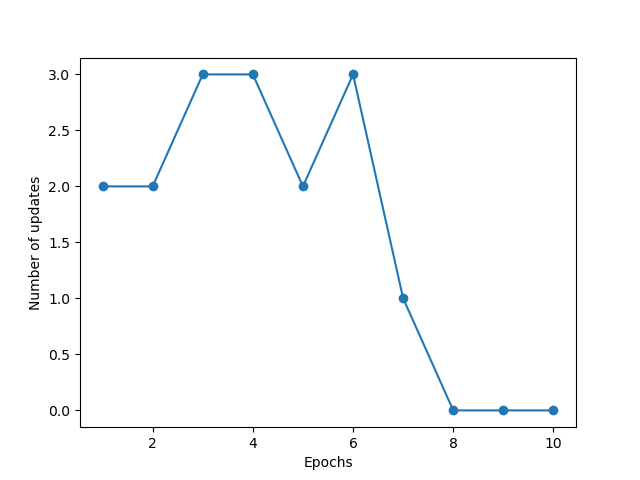
\includegraphics[width=0.7\textwidth]{png/Figure_1.png}
\end{center}

\newpage

\section{Question 2: Learning Axis-Aligned Rectangle with a Perceptron}
\subsection{Answers}
\begin{itemize}
    \item \textbf{Convergence Observations (100 samples, $\mathbf{w}^{(0)} = [0.25, 0.125, 0.0625],\, b^{(0)}=0$, $\eta=0.1$):}
    \begin{enumerate}
        \item At 10, 20, 30, and 100 epochs, the perceptron did not converge completely (number of updates did not reach zero), indicating that the data is not linearly separable. 
        \item As the number of epochs increased, misclassification errors decreased for a while but plateaued, suggesting the limit of what can be achieved with a linear decision boundary.
    \end{enumerate}
    
    \item \textbf{Train/Test Split Analysis:}
    \begin{enumerate}
        \item Training on first 60 samples for 10 epochs, and then evaluating on eight groups of 5 samples from the remaining 40 showed an error proportion below 0.2 on at least \textbf{[number]} group(s).
        \item Therefore, the model achieved acceptable performance in some splits, but not in all.
    \end{enumerate}
\end{itemize}

\subsection{Supporting Code}
\begin{verbatim}
# Copy your main code for training and producing outputs here, if required by instructions
\end{verbatim}

\subsection{Figure}
% \begin{center}
%   \includegraphics[width=0.7\textwidth]{png/rectangle_result.png}
% \end{center}

\newpage

% Repeat analogously for Question 3 (Adaline - Boolean functions) and Question 4 (Adaline - Rectangle)

\section*{References}
\begin{itemize}
    \item Machine Learning code and figures: adapted from Chapter 2 of ``Machine Learning with PyTorch and Scikit-Learn'', Sebastian Raschka (GitHub code).
    \item Any other references, acknowledgements, or credits.
\end{itemize}

\end{document}
